%%%%%%%%%%%%%%%%%%%%%%%%%%%%%%%%%%%%%%%%%%%%%%%%%%%%%%%%%%%%%%%%%%
%%%%%%%% ICML 2014 EXAMPLE LATEX SUBMISSION FILE %%%%%%%%%%%%%%%%%
%%%%%%%%%%%%%%%%%%%%%%%%%%%%%%%%%%%%%%%%%%%%%%%%%%%%%%%%%%%%%%%%%%

% Use the following line _only_ if you're still using LaTeX 2.09.
%\documentstyle[icml2014,epsf,natbib]{article}
% If you rely on Latex2e packages, like most moden people use this:
\documentclass{article}

% use Times
\usepackage{times}
% For figures
\usepackage{graphicx} % more modern
%\usepackage{epsfig} % less modern
%\usepackage{subfigure}

% For citations
\usepackage{natbib}

% For algorithms
\usepackage{algorithm}
\usepackage{algorithmic}

% As of 2011, we use the hyperref package to produce hyperlinks in the
% resulting PDF.  If this breaks your system, please commend out the
% following usepackage line and replace \usepackage{icml2014} with
%\usepackage[nohyperref]{icml2014} above.
\usepackage{hyperref}

% Packages hyperref and algorithmic misbehave sometimes.  We can fix
% this with the following command.
\newcommand{\theHalgorithm}{\arabic{algorithm}}

% Employ the following version of the ``usepackage'' statement for
% submitting the draft version of the paper for review.  This will set
% the note in the first column to ``Under review.  Do not distribute.''
\usepackage[accepted]{icml2014} 


% The \icmltitle you define below is probably too long as a header.
% Therefore, a short form for the running title is supplied here:
\icmltitlerunning{Objects Recognization Based on SOG with SVM}

\begin{document} 

\twocolumn[
\icmltitle{Objects Recognization Based on SOG with SVM\\Final Report for CIS 519}

% It is OKAY to include author information, even for blind
% submissions: the style file will automatically remove it for you
% unless you've provided the [accepted] option to the icml2014
% package.
\icmlauthor{Shangyi Cheng}{shangyi@seas.upenn.edu}
\icmlauthor{Yao Chu}{chuyao@seas.upenn.edu}
\icmlauthor{Chenyang Zhao}{chzhao@seas.upenn.edu}

% You may provide any keywords that you 
% find helpful for describing your paper; these are used to populate 
% the "keywords" metadata in the PDF but will not be shown in the document
\icmlkeywords{machine learning, circle detection, feature extraction, objects recognization, neural network}

\vskip 0.3in
]

\begin{abstract} 
We studied the question of object recognization using histograms of oriented gradients (HOG) with support vector machine (SVM) with Gaussian Kernel on ball detection as a test case. After reviewing several existing methods for feature extraction, our project verified that HOG performs well in ball recognization. We show the whole process from choosing regions of interest manually, extracting features from these regions, using principal component analysis (PCA) to reduce dimension of the  dataset and then applying SVM with Gaussian kernel to do the classification.   


\end{abstract}


\section{Introduction}
The target for this project is to detect the object of our interest and give the label for given images. The dataset we used are images of four kinds of balls from Caltech 256(Griffin, G. Holub, AD. Perona, P.), which contain 98 images of golf in the folder ``088.golf-ball'', 174 images of soccer ball in ``193.soccer-ball'', 104 images of bowling-ball in ``017.bowling-ball'' and 98 images of tennis ball in ``216.tennis-ball''. As shown in Figure \ref{fig:introduction}, among images of the same kind(take soccer-ball as example), some of the images have a whole soccer in the middle and fill the image, while in other images(such as a photo of a soccer game), the soccer may cover a small portion in the corner, only part of a soccer or several soccers are contained. We decide to use the image with a single target occupying most of the image as the training set. So the first thing we need to do before training is to create such standard images for training from the raw dataset.

\begin{figure}[htp]
\centering
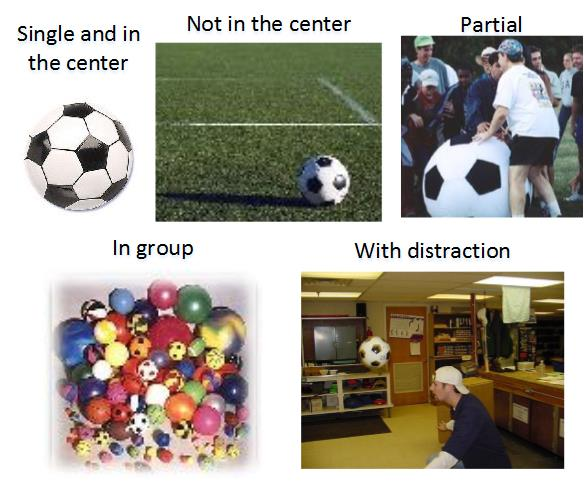
\includegraphics[width=0.4\textwidth]{Analysis_of_Available_Data.jpg}
\caption{Analysis of Available Data}
\label{fig:introduction}
\end{figure}

\section{Model Details} 

\subsection{Overview of the Method}
Inspired by the paper presented\cite{dalal2005histograms} by Navneet Dalal and Bill Triggs, we will try the method described in the paper. The interested region will be labeled manually for the training data. HOG features can be extracted from the interested region. Then SVM or other classifier will be applied to train the model. 

\subsection{Region of Interest (ROI) Selection}
Before we use the dataset directly as the training data, we need to select the region of interest which contains an object we would like our model to recognize. We tried several ways to select such region.\\
At the beginning, we considered using corner detection directly on the original image to select ROI and at the same time extract features. However, as shown in Figure \cite{crd}, extracting corner features based on the Harris Corner Detection and Adaptive Non-maximal Suppression method\ cite{brown2005multi} is not so helpful for following reasons: firstly, different pattern can be found in a single kind of balls so that geometric corner feature doesn't provide enough information for classification; secondly, the complicated background may generate large amount of features which are irrelevant to the ball.\\

\begin{figure}[htp]
\centering
	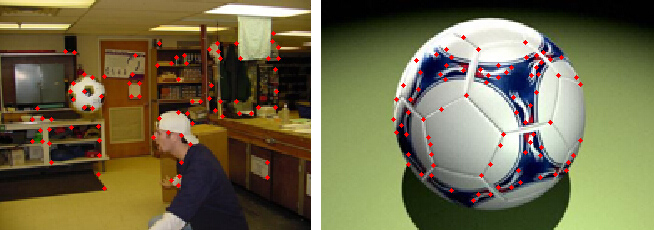
\includegraphics[width=0.4\textwidth]{CornerDetection.jpg}
\caption{Corner Detection Results}
\label{fig:crd}
\end{figure}

Then we tried several methods for circle detection including \cite{cirDetect1}, \cite{cirDetect2}, \cite{cirDetect3} to pick up the circular region and build the training set. One of the robustest approach is Circle Hough Transform(CHT), which takes the image $M$ and desired radius range $[r_{min},r_{max}]$ as inputs and return the positions of circle centers. As shown in Figure \cite{cird}, this method preforms good for the standard images with a single object occupyting the whole image but has a poor performance when there are other ball-like distractions such as heads and the tree holes on a bowling0ball, or only partial of the object, rather than a whole circle, appear on the image. It's also possible for CHT to return some position with high confidence for some circular patterns inside the ball. We found it was really hard to pick up the ROI just by the shape and without any referring to the features inside the region. \\

\begin{figure}[htp]
\centering
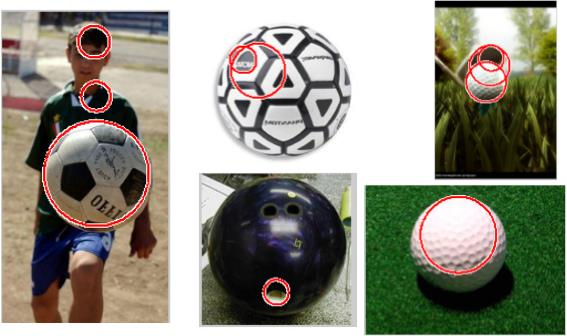
\includegraphics[width=0.4\textwidth]{circleDetection.jpg}
\caption{CHT Detection Results}
\label{fig:cird}
\end{figure}

Thus, we finally decided to pick up ROI for each image in dataset manually. To increase the number of instances in our training data, for each image, let the user chooses the ROI with a movable, resizable rectangle and position it interactively using the mouse. And then shift the area a little in one direction, thus a raw image will create at most nine images and at least one image for training. Finally, the picked area is resized to a $40 \times 40$ square. The algorithm is presented in Algorithm \ref{alg:Patch}.
\begin{algorithm}[tb]
   \caption{Select ROI Manually}
   \label{alg:Patch}
\begin{algorithmic}
   \STATE {\bfseries Input:} image $I$
   \STATE Initialize accumulator matrix $M = 0$.
   \FOR{each edge point$(i,j)$ in image $I$}
   \FOR{each point $(m,n)$ in image $I$}
   \IF{$r_{min}^2<(m-i)^2+(n-j)^2<r_{max}^2$}
   \STATE {$M(m,n) = M(m,n)+\phi_{m,n}$}
   \ENDIF
   \ENDFOR
   \ENDFOR
   \STATE {\bfseries Return:} positions of local maximum points in accumulator matrix $M$
\end{algorithmic}
\end{algorithm}\\

\subsection{PCA}
The number of features we get from last step using HOG is 900. Since the number of instances we use is about 4000 which is not large for 900 features, the training data is more likely to cause overfitting. On the other hand, to improve efficiency and decrease the time for training, it's necessary to reduce the dimension first. On the training dataset, we compute covariance matrix $\Sigma$ and data mean (average over all rows of $X$). Next, we choose the $d$ most important PCA basis vectors as the new training dataset. Then we should use $\Sigma$ and $X$ got previously on training dataset on the test data.






\section*{Acknowledgments} 
This project is supported by Upenn CIS 519. Thanks Eric Eaton and Xiaoxiang Hu for their instruction. Thanks MATLAB for providing so many useful toolbox.

\bibliography{report-ChengChuZhao}
\bibliographystyle{icml2014}

\end{document} 


